% Created by tikzDevice version 0.12.3.1 on 2021-07-11 22:21:44
% !TEX encoding = UTF-8 Unicode
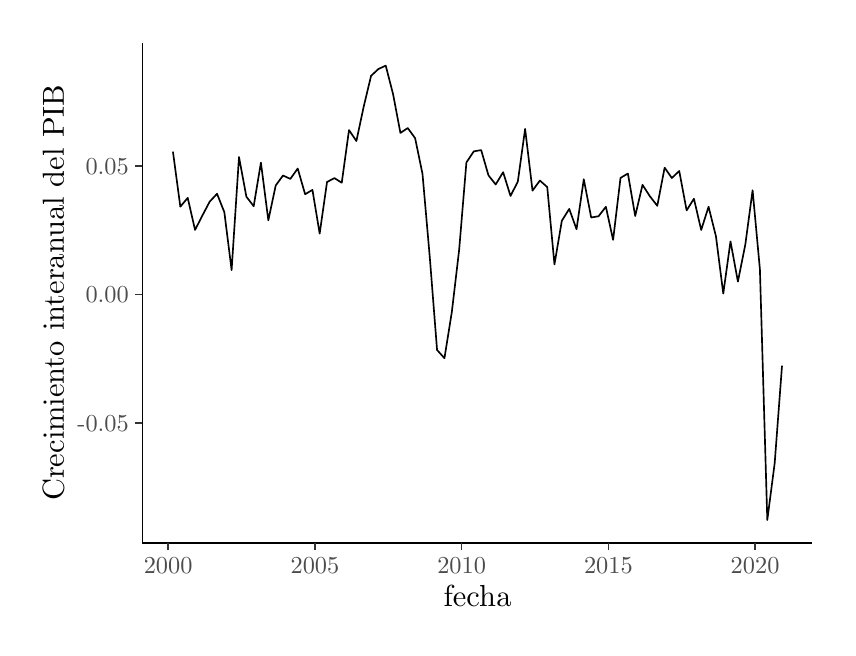
\begin{tikzpicture}[x=1pt,y=1pt]
\definecolor{fillColor}{RGB}{255,255,255}
\path[use as bounding box,fill=fillColor,fill opacity=0.00] (0,0) rectangle (289.08,216.81);
\begin{scope}
\path[clip] (  0.00,  0.00) rectangle (289.08,216.81);
\definecolor{drawColor}{RGB}{255,255,255}
\definecolor{fillColor}{RGB}{255,255,255}

\path[draw=drawColor,line width= 0.6pt,line join=round,line cap=round,fill=fillColor] (  0.00,  0.00) rectangle (289.08,216.81);
\end{scope}
\begin{scope}
\path[clip] ( 41.49, 30.69) rectangle (283.58,211.31);
\definecolor{fillColor}{RGB}{255,255,255}

\path[fill=fillColor] ( 41.49, 30.69) rectangle (283.58,211.31);
\definecolor{drawColor}{RGB}{0,0,0}

\path[draw=drawColor,line width= 0.6pt,line join=round] ( 52.49,172.02) --
	( 55.16,152.12) --
	( 57.83,155.31) --
	( 60.48,143.73) --
	( 63.09,148.85) --
	( 65.76,153.93) --
	( 68.43,156.79) --
	( 71.07,150.11) --
	( 73.69,129.22) --
	( 76.36,170.06) --
	( 79.03,155.73) --
	( 81.67,152.30) --
	( 84.28,168.04) --
	( 86.96,147.21) --
	( 89.63,159.79) --
	( 92.27,163.39) --
	( 94.91,162.16) --
	( 97.58,165.90) --
	(100.25,156.63) --
	(102.90,158.18) --
	(105.51,142.41) --
	(108.18,161.05) --
	(110.85,162.45) --
	(113.49,160.77) --
	(116.11,179.80) --
	(118.78,175.85) --
	(121.45,188.40) --
	(124.09,199.41) --
	(126.70,201.84) --
	(129.38,203.10) --
	(132.05,192.72) --
	(134.69,178.76) --
	(137.33,180.55) --
	(140.00,176.88) --
	(142.67,163.96) --
	(145.32,133.64) --
	(147.93,100.35) --
	(150.60, 97.38) --
	(153.27,114.08) --
	(155.91,136.51) --
	(158.53,168.08) --
	(161.20,172.11) --
	(163.87,172.57) --
	(166.51,163.43) --
	(169.12,160.16) --
	(171.80,164.59) --
	(174.47,156.01) --
	(177.11,161.16) --
	(179.75,180.23) --
	(182.42,157.93) --
	(185.09,161.56) --
	(187.74,159.22) --
	(190.35,131.26) --
	(193.02,147.04) --
	(195.69,151.31) --
	(198.33,143.99) --
	(200.95,162.03) --
	(203.62,148.22) --
	(206.29,148.67) --
	(208.93,152.09) --
	(211.54,140.12) --
	(214.22,162.52) --
	(216.89,164.11) --
	(219.53,148.75) --
	(222.17,160.01) --
	(224.84,155.88) --
	(227.51,152.45) --
	(230.16,166.21) --
	(232.77,162.49) --
	(235.44,165.02) --
	(238.11,150.78) --
	(240.75,155.00) --
	(243.37,143.71) --
	(246.04,152.11) --
	(248.71,141.37) --
	(251.35,120.71) --
	(253.96,139.58) --
	(256.64,125.06) --
	(259.31,138.37) --
	(261.95,158.06) --
	(264.59,129.50) --
	(267.26, 38.90) --
	(269.93, 59.46) --
	(272.58, 94.66);
\end{scope}
\begin{scope}
\path[clip] (  0.00,  0.00) rectangle (289.08,216.81);
\definecolor{drawColor}{RGB}{0,0,0}

\path[draw=drawColor,line width= 0.6pt,line join=round] ( 41.49, 30.69) --
	( 41.49,211.31);
\end{scope}
\begin{scope}
\path[clip] (  0.00,  0.00) rectangle (289.08,216.81);
\definecolor{drawColor}{gray}{0.30}

\node[text=drawColor,anchor=base east,inner sep=0pt, outer sep=0pt, scale=  0.88] at ( 36.54, 70.97) {-0.05};

\node[text=drawColor,anchor=base east,inner sep=0pt, outer sep=0pt, scale=  0.88] at ( 36.54,117.42) {0.00};

\node[text=drawColor,anchor=base east,inner sep=0pt, outer sep=0pt, scale=  0.88] at ( 36.54,163.87) {0.05};
\end{scope}
\begin{scope}
\path[clip] (  0.00,  0.00) rectangle (289.08,216.81);
\definecolor{drawColor}{gray}{0.20}

\path[draw=drawColor,line width= 0.6pt,line join=round] ( 38.74, 74.00) --
	( 41.49, 74.00);

\path[draw=drawColor,line width= 0.6pt,line join=round] ( 38.74,120.45) --
	( 41.49,120.45);

\path[draw=drawColor,line width= 0.6pt,line join=round] ( 38.74,166.90) --
	( 41.49,166.90);
\end{scope}
\begin{scope}
\path[clip] (  0.00,  0.00) rectangle (289.08,216.81);
\definecolor{drawColor}{RGB}{0,0,0}

\path[draw=drawColor,line width= 0.6pt,line join=round] ( 41.49, 30.69) --
	(283.58, 30.69);
\end{scope}
\begin{scope}
\path[clip] (  0.00,  0.00) rectangle (289.08,216.81);
\definecolor{drawColor}{gray}{0.20}

\path[draw=drawColor,line width= 0.6pt,line join=round] ( 50.75, 27.94) --
	( 50.75, 30.69);

\path[draw=drawColor,line width= 0.6pt,line join=round] (103.80, 27.94) --
	(103.80, 30.69);

\path[draw=drawColor,line width= 0.6pt,line join=round] (156.81, 27.94) --
	(156.81, 30.69);

\path[draw=drawColor,line width= 0.6pt,line join=round] (209.83, 27.94) --
	(209.83, 30.69);

\path[draw=drawColor,line width= 0.6pt,line join=round] (262.85, 27.94) --
	(262.85, 30.69);
\end{scope}
\begin{scope}
\path[clip] (  0.00,  0.00) rectangle (289.08,216.81);
\definecolor{drawColor}{gray}{0.30}

\node[text=drawColor,anchor=base,inner sep=0pt, outer sep=0pt, scale=  0.88] at ( 50.75, 19.68) {2000};

\node[text=drawColor,anchor=base,inner sep=0pt, outer sep=0pt, scale=  0.88] at (103.80, 19.68) {2005};

\node[text=drawColor,anchor=base,inner sep=0pt, outer sep=0pt, scale=  0.88] at (156.81, 19.68) {2010};

\node[text=drawColor,anchor=base,inner sep=0pt, outer sep=0pt, scale=  0.88] at (209.83, 19.68) {2015};

\node[text=drawColor,anchor=base,inner sep=0pt, outer sep=0pt, scale=  0.88] at (262.85, 19.68) {2020};
\end{scope}
\begin{scope}
\path[clip] (  0.00,  0.00) rectangle (289.08,216.81);
\definecolor{drawColor}{RGB}{0,0,0}

\node[text=drawColor,anchor=base,inner sep=0pt, outer sep=0pt, scale=  1.10] at (162.53,  7.64) {fecha};
\end{scope}
\begin{scope}
\path[clip] (  0.00,  0.00) rectangle (289.08,216.81);
\definecolor{drawColor}{RGB}{0,0,0}

\node[text=drawColor,rotate= 90.00,anchor=base,inner sep=0pt, outer sep=0pt, scale=  1.10] at ( 13.08,121.00) {Crecimiento interanual del PIB};
\end{scope}
\end{tikzpicture}
